\section{Les sociétés de contrôle}

\paragraph{Une portée personnelle}

\paragraph{} L'utilisation d'un service est de nos jours synonyme de production et donc collecte de données ; ne dit-on
pas que si un service est gratuit, c'est que ses utilisateurs en sont les produits ? Dès lors nous ne sommes plus maîtres
des informations que nous publions, qui peuvent être vendues ou récupérées à des fins diverses : publicité et marketing
ciblés en sont des exemples bien connus.

\paragraph{} Mais les données ne sont pas uniquement utilisées de manière ciblée. Le développement ces dernières années 
des \emph{Smart Cities} donne naissance à des initiatives auparavant impensables. Ainsi la ville de New York s'est-elle
dôtée d'un tableau de bord \cite{ProgrammableCity1} aggrégeant l'ensemble des sources de données à sa disposition pour 
mettre en exergue de nombreux indicateurs : fluctuation des prix de l'immobilier, évolution du nombre de plaintes pour 
tapage nocturne par quartier, hygiène des rues, état de la circulation aux différentes heures de la journée...
Toutes ces données dont \emph{nous} sommes la source sont ainsi mises au service de la ville.

\paragraph{} \emph{The Programmable City} \cite{ProgrammableCity0} est un projet proposant de mettre la technologie au
service de l'urbanisme. Une infrastructure et un ensemble de programmes nous permettent de piloter et d'être à l'écoute
de la ville, qui bénéficie au quotidien d'une attention nouvelle : on crée alors un cercle vertueux. Le site
\url{http://DublinDashboard.ie/} est une mise en application de ces concepts pour la ville de Dublin, proposant des
dizaines de sources de données visualisables concernant l'agglomération. D'autres initiatives, comme celle de SideWalk Labs
à Toronto \cite{ProgrammableCity3}, visent à réinventer la ville pour remettre l'humain au c\oe{}ur des processus de
décision en utilisant les nouvelles technologies et les données générées pour améliorer de manière continue les services
qu'elle fournit.

\begin{figure}[h]
    \centering
    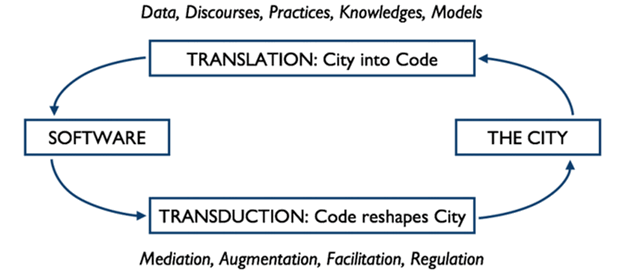
\includegraphics[width=300px]{chapters/01/images/programmable_city.png}
    \caption{\label{programmable_city} Le cycle de transduction des \emph{Programmable Cities}}
\end{figure}

\paragraph{} Une donnée, ce n'est rien de plus que de l'information numérisée. Là où ces bases de données publiques
émanant de structures privées ne nous étonnent en rien - car nous sommes \emph{habitués} à les alimenter, comme l'application
Uber Movement permettant d'analyser les trajets effectués via le service Uber -, il est important de comprendre
qu'elles ne diffèrent pas de celles de nos services publics. Ce n'est qu'avec l'adoption progressive de l'\emph{Open
Data} que ces derniers se sont petit à petit ouverts au développement d'applications exploitant toutes sortes de données. 

\paragraph{} Bien évidemment, les \emph{Open Data} et autres sources de données des \emph{Smart Cities} ne sont pas
constituées de données personnelles - c'est à dire d'informations permettant d'identifier de manière directe ou non une 
personne physique \cite{PersonalData0}. Mais cela est-il réellement différent ? Ainsi la société Hitachi a-t-elle développé
en 2015 un système de prévention des crimes et délits reposant sur du machine learning \cite{ProgrammableCity2}. Une quantité
astronomique de données de toutes sortes est nécessaire pour alimenter le système, des mouvements de population aux 
antécédents de crimes enregistrés dans les zones sous surveillance. Ne peut-on pas alors craindre de voir une zone 
démographique désertée suite à un incident car son \emph{coefficient de criminalité} aura augmenté, rebutant nouveaux
résidents et jeunes parents à s'y installer ?

\paragraph{} La finalité de ces systèmes peut être réduite à cette simple question : se savoir surveillé restreint-il
les instincts pervers, ou au contraire cela les désinhibe-t-il ?

\paragraph{} \emph{Veiller} nous vient du latin classique \emph{vigilare} \guillemotleft être éveillé, être attentif, sur
ses gardes \guillemotright, mais aussi \guillemotleft entourer de soins \guillemotright \cite{Surveillance0}. Le préfixé
\emph{Surveiller} (XVI\up{ème} siècle) signifie alors \guillemotleft contrôler, observer avec attention \guillemotright.
Être \emph{sous la surveillance de}, c'est être \emph{observé par} mais aussi \emph{contrôlé par}, c'est-à-dire subordonné
directement ou indirectement à quelquechose ou quelqu'un.

\paragraph{} L'\emph{instinct} vient du latin \emph{instinctus}, qui dispose d'un double sens. En latin classique, il 
signifie \guillemotleft instigation, excitation, impulsion \guillemotright, et en latin chrétien \guillemotleft penchant,
tendance naturelle \guillemotright \cite{Instinct0}. Théorisé par les philosophes, le mot désigne pour Montaigne (XVI\up{ème} siècle) 
\guillemotleft l'ensemble des pulsions naturelles qui régissent le comportement animal ou humain \guillemotright (cette 
notion de \emph{pulsion} se retrouve chez Freud avec le \emph{Trieb} allemand), tandis que Pascal (XVII\up{ème} siècle)
en fait \guillemotleft la faculté naturelle de sentir, de deviner \guillemotright.

\paragraph{} Enfin, \emph{pervertir} apparaît dans l'ancien français au XII\up{ème} siècle sous la forme \emph{purvertir} et est
dérivé du latin \emph{pervertire} ; \emph{per-} \guillemotleft l'action de \guillemotright, et \emph{vertere} \guillemotleft
tourner, verser \guillemotright : il signifie alors \guillemotleft mettre sens dessus-dessous, faire mal tourner \guillemotright
\cite{Pervers0}. Dans le langage religieux, le \emph{pervers} est une personne \guillemotleft portée à faire le mal \guillemotright
et est alors synonyme de \emph{dur}, \emph{cruel}, \emph{furieux} (XIII\up{ème} siècle). En français moderne, il désigne 
\guillemotleft la personne qui montre une tendance pathologique à accomplir des actes immoraux \guillemotright, voire même
celle \guillemotleft dont les \emph{pulsions} ne sont pas fixées \guillemotright pour les psychanalystes.

\paragraph{} Qu'entend-on donc par \emph{instincts pervers} ? L'instinct, c'est la pulsion ; la perversion, c'est l'absence
de fixation. Or \emph{fixer}, c'est \guillemotleft établir d'une manière durable dans une position déterminée \guillemotright \cite{Fixe0}.
Les instincts pervers, ce sont donc toutes les pulsions "hors norme", hors du cadre déterminé, en décalage avec la réalité
telle qu'elle est acceptée (ou définie) par le groupe ; la perversion n'a de sens que dans un contexte sociétal.

\paragraph{} Nous touchons donc bien à la raison d'être des sociétés de contrôle : restreindre les instincts pervers c'est
normaliser, niveller par le bas, et l'ensemble des systèmes de surveillance contribuent à accentuer ce phénomène \cite{SocialMedia0}.
\emph{Se savoir surveillé}, ce n'est rien de plus que posséder un compte sur un réseau social : on y incarne à tour de
\emph{rôle} juge, avocat et accusé, et l'on s'accroche à l'idée illusoire que l'on n'a pas perdu le \emph{contrôle}.

\paragraph{} Vaudrait-il mieux alors vivre dans une société où sévissent quelques individus extrêmement pervers, ou dans
une société \emph{lissée}, \emph{amortie}, \emph{normalisée} ? Le modèle panoptique (voir \ref{panoptique}, page \pageref{panoptique})
ne s'est jamais généralisé car il était trop évident, manquant de subtilité. Les technologies ont permis de mettre en application
le modèle du \emph{surveilleur-surveillé}.


\paragraph{Évolution du partage}

\paragraph{} Évolution du partage : les réseaux sociaux, quelles moeurs ? Catégoriees d'âges ? Sociaux-professionnelles ?
Quelle forme de contrôle incarnée par notre prototype ? À qui est-il destiné ? Pour quelles utilisations ?
La place de l'information/désinformation ?


\paragraph{L'individu technique}

\paragraph{} Comment les modèles de sociétés nous ont-ils amené à réfléchir l'individu en termes technologiques ?